\scanpage{361}
\hfill EZ \deleted{2}3
\[
f\in H^n(X,A)\quad\Longrightarrow\quad Pf\in{}_{\Sigma_n}H^{pn}(E\Sigma_n\times X^p,A)
\quad\Longrightarrow\quad\Delta Pf\in H^{pn}(K(\Sigma_p,1)\times X,A)
\]
\diagram{\begin{tikzcd}[column sep=large,row sep=small]
&\Vert\\
&H^{\unsure{*|\lambda}}(K(\Sigma_p,1)\otimes_{\mathbb F_p}H^*(X,A)\arrow[ddd,start anchor=south east,end anchor=north east,sloped]\\
&\unsure{\varphi|0}\quad\deleted{\unsure{E\Sigma_1|E\Sigma_n}}\\
\unsure{e|\mathcal E}_{\alpha}\in H_{\alpha}(K(\Sigma_p,1))&{}\\
&D_i x\in H^{pn-i}(X,A)
\end{tikzcd}}
\[
\underline{P^i x}=(-1)^{(\ )}D_{f(i)}.
\]
Ce reindexage est ce qui donne la formule de Cartan

En fait on considere $\mathbb Z_p\subset\Sigma_p$ et on travaille avec la coh du groupe cyclique
\figure{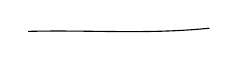
\begin{tikzpicture}\draw (0,0) .. controls (.8,.02) and (1.5,-.04) .. (2.3,.04);\end{tikzpicture}}
\mspage{362}
